%!TEX root = ../DigPro2.tex
\section{Morphological Image Processing\buch{Ch. 9}\buchSeite{635-698}}

\subsection{Set Theory}
\begin{multicols}{2}
\subsubsection{Reflection\buchSeite{637}}
\[
	\hat{B} = \{w | w = -b,\quad \text{for} \quad b \in B \}
\]


\subsubsection{Translation\buchSeite{637}}
\[
	(B)_z = \{ c | c = b + z,\quad \text{for} \quad b \in B\}
\]

\subsection{Erosion and Dilation}
\subsubsection{Erosion\buchSeite{639}}
With A and B as sets in $Z^2$, the erosion of A by B is defined as
\[
	A \ominus B = \{z|(B)_z \subseteq A  \}
\]

This is the set of all translations by z such that the set B is still a subset of A.

Equivalently, if B must be contained in A, it is not allowed to intersect with the background:
\[
	A \ominus B = \{z|(B)_z \cap A^c = \varnothing  \}
\]


\subsubsection{Dilation\buchSeite{641}}
With A and B as sets in $Z^2$, the dilation of A by B is defined as
\[
	A \oplus B = \{z |(\hat{B})_z \cap A \neq \varnothing \}
\]
This is the set of all translations by z such that the set B reflected about its origin has at least one overlap with the set A.

Equivalently, since the intersection is not allowed to be empty and all elements in it must be from A:
\[
	A \oplus B = \{z | [(\hat{B})_z \cap A] \subseteq A \}
\]


\subsubsection{Duality erosion/dilation\buchSeite{644}}
Erosion and dilation are dual:
\[
	(A  \ominus B)^c = A^c \oplus \hat{B}
\]
\[
	(A \oplus B)^c = A^c \ominus \hat{B}
\]

\end{multicols}
\subsection{Opening and Closing}
\subsubsection{Opening and closing\buchSeite{644}}
The \emph{opening} of A by B is defined: (first erosion then dilation)
\[
	A \circ B = (A \ominus B) \oplus B
\]

The \emph{closing} of A by B is defined: (first dilation then erosion)
\[
	A  \bullet B = (A \oplus B) \ominus B
\]

Opening and closing are dual operations:
\[
	(A  \bullet B)^c = (A^c \circ \hat{B})
\]
\[
	(A \circ B)^c = (A^c \bullet \hat{B})
\]

The \textbf{opening} operation satisfies the following properties:
\begin{enumerate}[label=\textbf{(\alph*)}]
	\item $A \circ B$ is a subset (subimage) of $A$.
	\item If $C$ is a subset of $D$, then $C \circ B$ is a subset of $D \circ B$.
	\item $(A \circ B) \circ B = A \circ B$
\end{enumerate}

The \textbf{closing} operation satisfies the following properties:
\begin{enumerate}[label=\textbf{(\alph*)}]
	\item $A$ is a subset (subimage) of $A \bullet B$.
	\item If $C$ is a subset of $D$, then $C \bullet B$ is a subset of $D \bullet B$.
	\item $(A \bullet B) \bullet B = A \bullet B$
\end{enumerate}

\begin{figure}[h!]
	\centering
	\begin{subfigure}[b]{0.45\textwidth}
		\centering
		\adjustbox{scale=0.5}{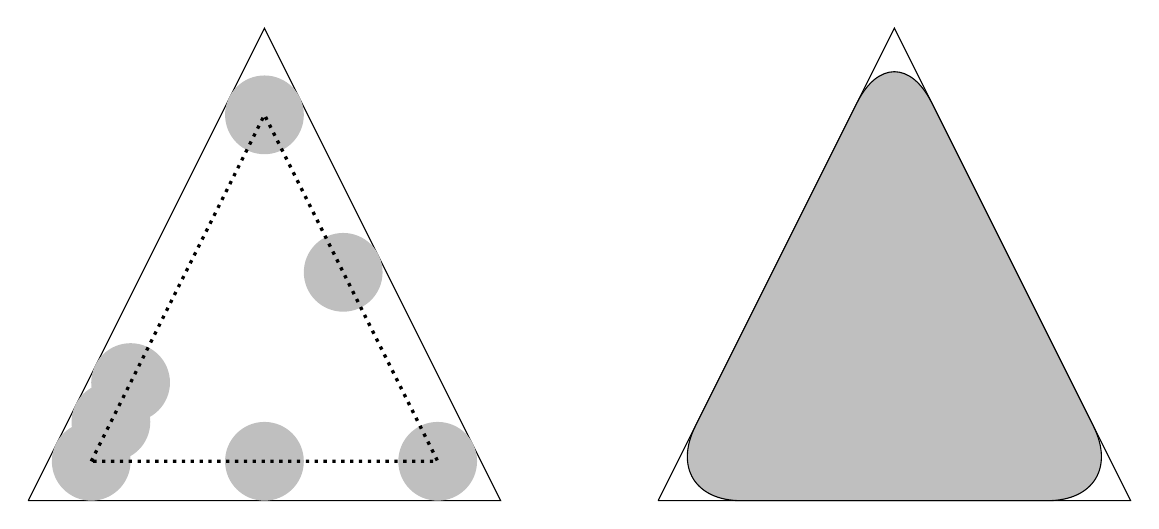
\begin{tikzpicture}
%linkes dreieck
\draw (0,0) -- (3,6) -- (6,0) -- (0,0);
\fill [lightgray] (0.8,0.5) circle (0.5);
\fill [lightgray] (1.05,1) circle (0.5);
\fill [lightgray] (1.3,1.5) circle (0.5);
\fill [lightgray] (3,4.9) circle (0.5);
\fill [lightgray] (4,2.9) circle (0.5);
\fill [lightgray] (5.2,0.5) circle (0.5);
\fill [lightgray] (3,0.5) circle (0.5);
\draw [dotted, very thick] (0.8,0.5) -- (3,4.9) -- (5.2,0.5) -- (0.8,0.5);

\draw (8,0) -- (11,6) -- (14,0) -- (8,0);
\draw [rounded corners=30pt, fill=lightgray] (9,2) -- (11,6) -- (14,0) -- (8,0) -- (9,2);

\end{tikzpicture}}
		\caption{Opening}
	\end{subfigure}
	\begin{subfigure}[b]{0.45\textwidth}
		\centering
		\adjustbox{scale=0.5}{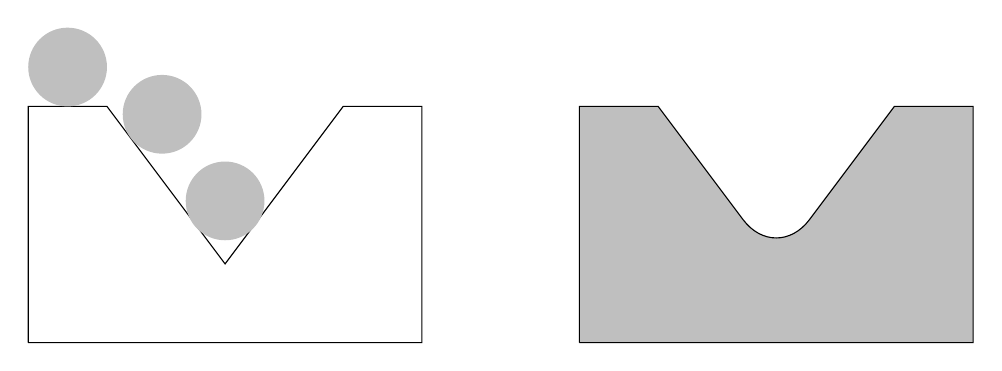
\begin{tikzpicture}

\draw (0,0) -- (0,3) -- (1,3) -- (2.5,1) -- (4,3) -- (5,3) -- (5,0) -- (0,0);
\fill [lightgray] (0.5,3.5) circle (0.5);
\fill [lightgray] (1.7,2.9) circle (0.5);
\fill [lightgray] (2.5,1.8) circle (0.5);

\draw [fill=lightgray] (7,0) -- (7,3) -- (8,3) [rounded corners=20pt] -- (9.5,1) [rounded corners=0] -- (11,3) -- (12,3) -- (12,0) -- (7,0);

\end{tikzpicture}}
		\caption{Closing}
	\end{subfigure}
	\caption{Geometrical interpretation of the opening and closing transformations}
\end{figure}


\subsection{The hit-or-miss transform\buchSeite{648}}
The hit-or-miss transform is a basic tool for shape detection. Basic idea:
\begin{itemize}
	\item Through erosion of the image by the object, possible locations for the object in the image are left, since elements smaller than the objects disappear

	\item Through erosion of the background of the image with the local background of the object, possible locations for the object in the image are left

	\item The intersection of these possible locations result in a reliable  detection of the object location
	\[
		A \circledast B = (A \ominus D) \cap [ A^c \ominus (W-D)]
	\]

	\item In general, if B1 is the object and B2 is the corresponding background this can be written
	\[
		A \circledast B = (A \ominus B_1)\cap (A^c \ominus B_2)
	\]
\end{itemize}


\subsection{Some basic morphological algorithms\buchSeite{652}}
\subsubsection{Boundary Extraction\buchSeite{653}}
\begin{multicols}{2}
	\begin{align*}
		\beta(A)=A-(A\ominus B)
	\end{align*}
	The mask \quad \adjustbox{max width=1cm}{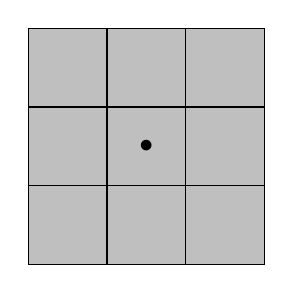
\begin{tikzpicture}
\draw [fill=lightgray] (0,0) rectangle  (3,3);
\node at (1.5,1.5) {$\bullet$};
\foreach \x in {0,1,2,3} {
\draw (\x,0) -- (\x,3);
\draw (0,\x) -- (3,\x);}
\end{tikzpicture}}
	\quad leads to a 1 pixel thick boundary
\end{multicols}

\subsubsection{Hole Filling\buchSeite{653}}
\begin{multicols}{2}
To fill a hole, a seed inside the connected border is needed, i.e., in an empty array $X_0$, the seed point is set to 1.
\begin{align*}
X_k=(X_{k-1}\oplus B)\cap A^c && k=1,2,3,\ldots
\end{align*}

Usual mask: \adjustbox{max width=1cm}{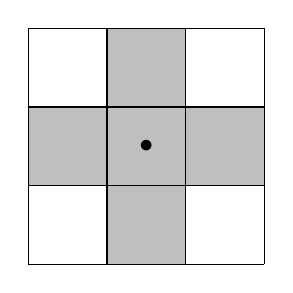
\begin{tikzpicture}
\draw [fill=lightgray] (0,1) rectangle  (3,2);
\draw [fill=lightgray] (1,0) rectangle  (2,3);
\node at (1.5,1.5) {$\bullet$};
\foreach \x in {0,1,2,3} {
\draw (\x,0) -- (\x,3);
\draw (0,\x) -- (3,\x);}
\end{tikzpicture}} \\

The dilation is forced to stay inside the connected border with $\cap A^c$.The iteration can stop, when $X_k = X_{k-1}$.
\end{multicols}

\subsubsection{Extraction of Connected Components\buchSeite{655}}
\begin{multicols}{2}
Initial array ($X_0$) contains a 1 in the region of the connected component.
\begin{align*}
X_k=(X_{k-1}\oplus B)\cap A && k=1,2,3,\ldots
\end{align*}
The iteration can stop, when $X_k = X_{k-1}$. \\
The mask \quad \adjustbox{max width=1cm}{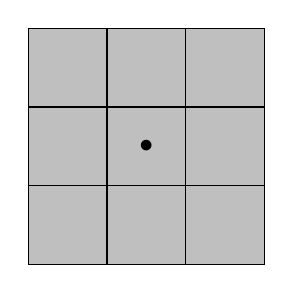
\begin{tikzpicture}
\draw [fill=lightgray] (0,0) rectangle  (3,3);
\node at (1.5,1.5) {$\bullet$};
\foreach \x in {0,1,2,3} {
\draw (\x,0) -- (\x,3);
\draw (0,\x) -- (3,\x);}
\end{tikzpicture}}
\quad leads to 8-connected regions.
\end{multicols}

\subsubsection{Convex hull\buchSeite{657}}
\begin{itemize}
\item The convex hull H of a set S is the smalles convex set containing S.
\item H-S is called the convex deficiency of S
\end{itemize}
The convex hull is constructed with a convex hull with four structuring elements. (x = don't care)
\begin{figure}[h]
	\centering
	\begin{subfigure}[b]{0.2\textwidth}
		\centering
		\adjustbox{scale=0.5}{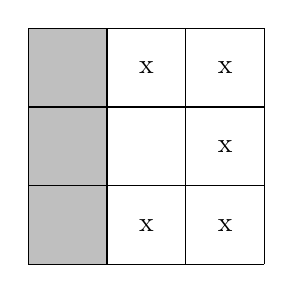
\begin{tikzpicture}
\draw [fill=lightgray] (0,0) rectangle  (1,3);
\foreach \x in {0,1,2,3} {
\draw (\x,0) -- (\x,3);
\draw (0,\x) -- (3,\x);}
\node at (1.5,0.5) {x};
\node at (2.5,0.5) {x};
\node at (2.5,1.5) {x};
\node at (2.5,2.5) {x};
\node at (1.5,2.5) {x};
\end{tikzpicture}}
		\caption{$B^1$}
	\end{subfigure}
	\begin{subfigure}[b]{0.2\textwidth}
		\centering
		\adjustbox{scale=0.5, angle=270}{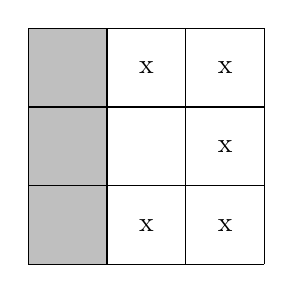
\begin{tikzpicture}
\draw [fill=lightgray] (0,0) rectangle  (1,3);
\foreach \x in {0,1,2,3} {
\draw (\x,0) -- (\x,3);
\draw (0,\x) -- (3,\x);}
\node at (1.5,0.5) {x};
\node at (2.5,0.5) {x};
\node at (2.5,1.5) {x};
\node at (2.5,2.5) {x};
\node at (1.5,2.5) {x};
\end{tikzpicture}}
		\caption{$B^2$}
	\end{subfigure}
	\begin{subfigure}[b]{0.2\textwidth}
		\centering
		\adjustbox{scale=0.5, angle=180}{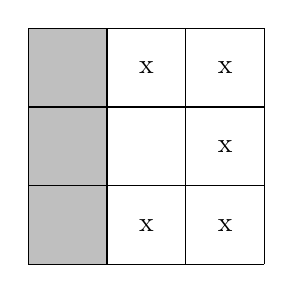
\begin{tikzpicture}
\draw [fill=lightgray] (0,0) rectangle  (1,3);
\foreach \x in {0,1,2,3} {
\draw (\x,0) -- (\x,3);
\draw (0,\x) -- (3,\x);}
\node at (1.5,0.5) {x};
\node at (2.5,0.5) {x};
\node at (2.5,1.5) {x};
\node at (2.5,2.5) {x};
\node at (1.5,2.5) {x};
\end{tikzpicture}}
		\caption{$B^3$}
	\end{subfigure}
	\begin{subfigure}[b]{0.2\textwidth}
		\centering
		\adjustbox{scale=0.5, angle=90}{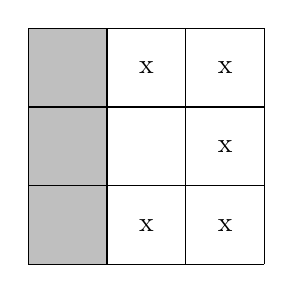
\begin{tikzpicture}
\draw [fill=lightgray] (0,0) rectangle  (1,3);
\foreach \x in {0,1,2,3} {
\draw (\x,0) -- (\x,3);
\draw (0,\x) -- (3,\x);}
\node at (1.5,0.5) {x};
\node at (2.5,0.5) {x};
\node at (2.5,1.5) {x};
\node at (2.5,2.5) {x};
\node at (1.5,2.5) {x};
\end{tikzpicture}}
		\caption{$B^4$}
	\end{subfigure}
	\caption{Structuring elements for convex hull}
\end{figure}

\begin{align*}
	X_0^i &= A \\
	X_k^i &= (X_{k-1}^i \circledast B^i) \cup A & i &=1,2,3,4 \text{ and } k=1,2,3,\ldots \\
	\text{when } X_k^i &= X_{k-1}^i \longrightarrow D^i = X_k^i \\
	C(A) &= \bigcup\limits_{i=1}^4 D_i
\end{align*}

Note that the hit-or-miss transform $\circledast$ here is applied without background.

This algorithm does not guarantee that the found convex set is the convex hull, which has to be the smallest convex set containing the original object

The following additional constraints can be used:
\begin{itemize}
\item easiest is, that the convex hull is not allowed to grow beyond the original vertical and horizontal dimension
\item More complex constraints are possible, but at a higher computational cost
\end{itemize}

\subsubsection{Thinning\buchSeite{660}}
Thinning is the operation of making the foreground thinner.
\begin{figure}[h]
	\centering
	\begin{subfigure}[b]{0.45\textwidth}
		\centering
		\adjustbox{scale=0.5}{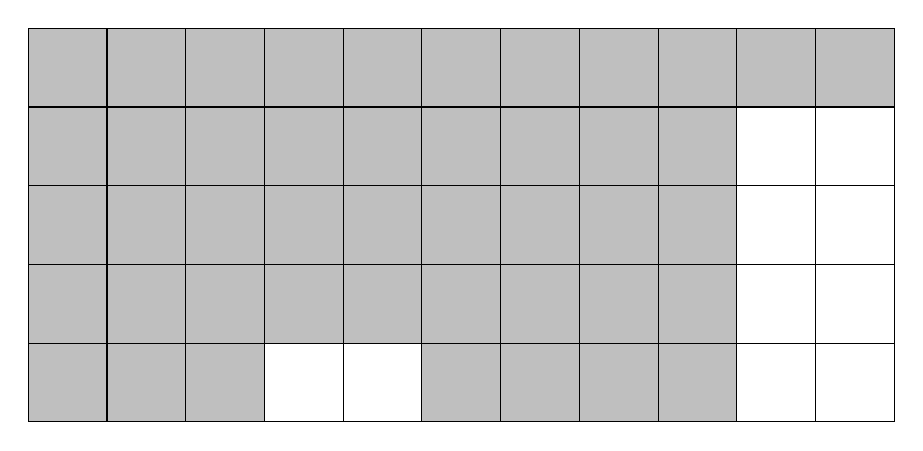
\begin{tikzpicture}
\draw[fill=lightgray] (0,5) rectangle (9,1);
\draw[fill=lightgray] (9,5) rectangle (11,4);
\draw[fill=lightgray] (5,1) rectangle (9,0);
\draw[fill=lightgray] (0,1) rectangle (3,0);
\foreach \x in {0,...,11} {
\draw (\x,0) -- (\x,5);}
\foreach \y in {0,...,5} {
\draw (0,\y) -- (11,\y);}
\end{tikzpicture}
}
		\caption{Original image}
	\end{subfigure}
	\begin{subfigure}[b]{0.45\textwidth}
		\centering
		\adjustbox{scale=0.5}{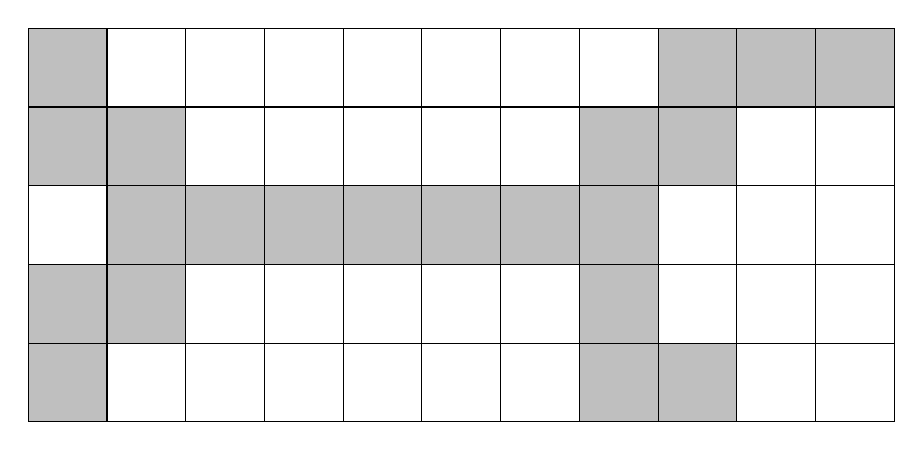
\begin{tikzpicture}
\draw[fill=lightgray] (1,3) rectangle (8,2);
\draw[fill=lightgray] (0,5) rectangle (1,4);
\draw[fill=lightgray] (0,4) rectangle (2,3);
\draw[fill=lightgray] (0,0) rectangle (1,1);
\draw[fill=lightgray] (0,1) rectangle (2,2);
\draw[fill=lightgray] (7,0) rectangle (9,1);
\draw[fill=lightgray] (7,1) rectangle (8,2);
\draw[fill=lightgray] (7,3) rectangle (9,4);
\draw[fill=lightgray] (8,4) rectangle (11,5);

\foreach \x in {0,...,11} {
\draw (\x,0) -- (\x,5);}
\foreach \y in {0,...,5} {
\draw (0,\y) -- (11,\y);}

\end{tikzpicture}}
		\caption{Thinned image}
	\end{subfigure}
	\caption{Thinning}
\end{figure}
	\[
		A \otimes  B = A - (A \circledast B)
	\]
Hit-or-miss transformation with rotating structuring elements. Note that the hit-or-miss is applied without background. \\

\begin{figure}[h]
	\centering
	\begin{subfigure}[b]{0.1\textwidth}
		\centering
		\adjustbox{scale=0.5}{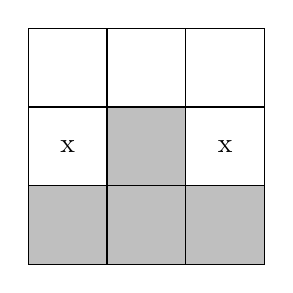
\begin{tikzpicture}
\draw [fill=lightgray] (0,0) rectangle  (3,1);
\draw [fill=lightgray] (1,1) rectangle  (2,2);
\foreach \x in {0,1,2,3} {
\draw (\x,0) -- (\x,3);
\draw (0,\x) -- (3,\x);}
\node at (0.5,1.5) {x};
\node at (2.5,1.5) {x};
\end{tikzpicture}}
		\caption{$B^1$}
	\end{subfigure}
	\begin{subfigure}[b]{0.1\textwidth}
		\centering
		\adjustbox{scale=0.5}{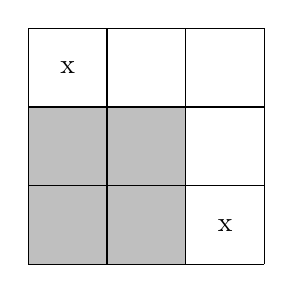
\begin{tikzpicture}
\draw [fill=lightgray] (0,0) rectangle  (2,2);
\foreach \x in {0,1,2,3} {
\draw (\x,0) -- (\x,3);
\draw (0,\x) -- (3,\x);}
\node at (0.5,2.5) {x};
\node at (2.5,0.5) {x};
\end{tikzpicture}}
		\caption{$B^2$}
	\end{subfigure}
	\begin{subfigure}[b]{0.1\textwidth}
		\centering
		\adjustbox{scale=0.5, angle=270}{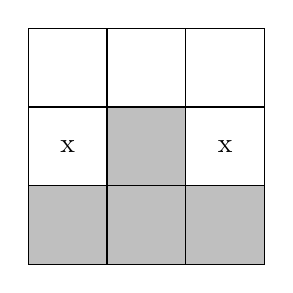
\begin{tikzpicture}
\draw [fill=lightgray] (0,0) rectangle  (3,1);
\draw [fill=lightgray] (1,1) rectangle  (2,2);
\foreach \x in {0,1,2,3} {
\draw (\x,0) -- (\x,3);
\draw (0,\x) -- (3,\x);}
\node at (0.5,1.5) {x};
\node at (2.5,1.5) {x};
\end{tikzpicture}}
		\caption{$B^3$}
	\end{subfigure}
	\begin{subfigure}[b]{0.1\textwidth}
		\centering
		\adjustbox{scale=0.5, angle=270}{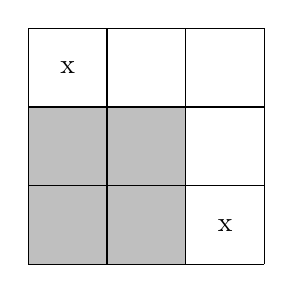
\begin{tikzpicture}
\draw [fill=lightgray] (0,0) rectangle  (2,2);
\foreach \x in {0,1,2,3} {
\draw (\x,0) -- (\x,3);
\draw (0,\x) -- (3,\x);}
\node at (0.5,2.5) {x};
\node at (2.5,0.5) {x};
\end{tikzpicture}}
		\caption{$B^4$}
	\end{subfigure}
	\begin{subfigure}[b]{0.1\textwidth}
		\centering
		\adjustbox{scale=0.5, angle=180}{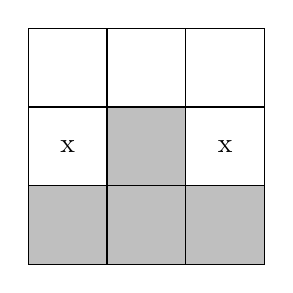
\begin{tikzpicture}
\draw [fill=lightgray] (0,0) rectangle  (3,1);
\draw [fill=lightgray] (1,1) rectangle  (2,2);
\foreach \x in {0,1,2,3} {
\draw (\x,0) -- (\x,3);
\draw (0,\x) -- (3,\x);}
\node at (0.5,1.5) {x};
\node at (2.5,1.5) {x};
\end{tikzpicture}}
		\caption{$B^5$}
	\end{subfigure}
	\begin{subfigure}[b]{0.1\textwidth}
		\centering
		\adjustbox{scale=0.5, angle=180}{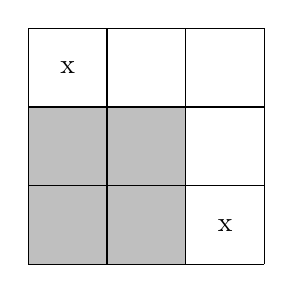
\begin{tikzpicture}
\draw [fill=lightgray] (0,0) rectangle  (2,2);
\foreach \x in {0,1,2,3} {
\draw (\x,0) -- (\x,3);
\draw (0,\x) -- (3,\x);}
\node at (0.5,2.5) {x};
\node at (2.5,0.5) {x};
\end{tikzpicture}}
		\caption{$B^6$}
	\end{subfigure}
	\begin{subfigure}[b]{0.1\textwidth}
		\centering
		\adjustbox{scale=0.5, angle=90}{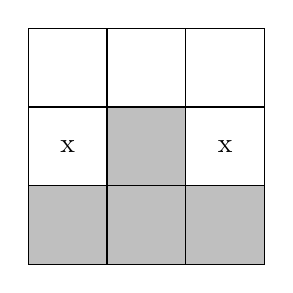
\begin{tikzpicture}
\draw [fill=lightgray] (0,0) rectangle  (3,1);
\draw [fill=lightgray] (1,1) rectangle  (2,2);
\foreach \x in {0,1,2,3} {
\draw (\x,0) -- (\x,3);
\draw (0,\x) -- (3,\x);}
\node at (0.5,1.5) {x};
\node at (2.5,1.5) {x};
\end{tikzpicture}}
		\caption{$B^7$}
	\end{subfigure}
	\begin{subfigure}[b]{0.1\textwidth}
		\centering
		\adjustbox{scale=0.5, angle=90}{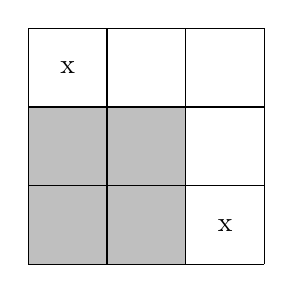
\begin{tikzpicture}
\draw [fill=lightgray] (0,0) rectangle  (2,2);
\foreach \x in {0,1,2,3} {
\draw (\x,0) -- (\x,3);
\draw (0,\x) -- (3,\x);}
\node at (0.5,2.5) {x};
\node at (2.5,0.5) {x};
\end{tikzpicture}}
		\caption{$B^8$}
	\end{subfigure}
	\caption{Thinning masks}
\end{figure}
	\[
		A \otimes  {B} = ((\ldots((A \otimes B^{1}) \otimes B^{2})\ldots) \otimes B^{n})
	\]

This is repeated until nothing changes anymore.

\subsubsection{Thickening\buchSeite{660}}
This is the morphological dual of thinning. It is implemented as thinning the background and then taking the complement.
Thickening can lead to disconnected points. These have to be removed by post-processing.

\subsubsection{Skeleton S(A)\buchSeite{662}}
\begin{figure}[h!]
\centering
\begin{subfigure}[b]{0.45\textwidth}
\centering
\adjustbox{scale=0.5}{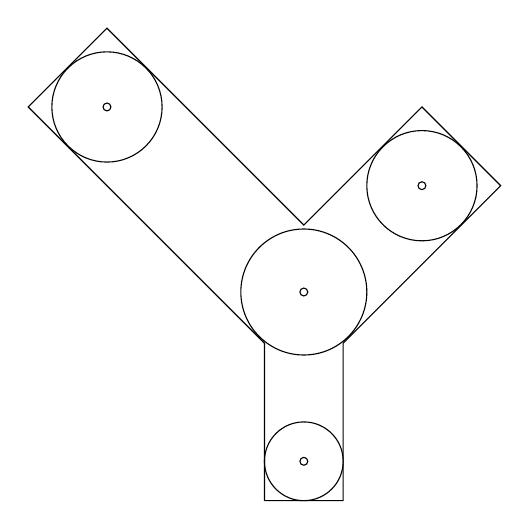
\begin{tikzpicture}
\draw (5,0) -- (6,0) -- (6,2) -- (8,4) -- (7,5) -- (5.5,3.5) -- (3,6) -- (2,5) -- (5,2) -- (5,0);
\draw (5.5,0.5) circle (0.5) circle (0.05);
\draw (3,5) circle (0.7) circle (0.05);
\draw (5.5,2.65) circle (0.8) circle (0.05);
\draw (7,4) circle (0.7) circle (0.05);
\end{tikzpicture}}
\caption{Positions of Maximum disks}
\end{subfigure}
\begin{subfigure}[b]{0.45\textwidth}
\centering
\adjustbox{scale=0.5}{\begin{tikzpicture}
\draw (5,0) -- (6,0) -- (6,2) -- (8,4) -- (7,5) -- (5.5,3.5) -- (3,6) -- (2,5) -- (5,2) -- (5,0);
\draw [dashed] (5,0) -- (5.5,0.5) -- (6,0);
\draw [dashed] (2,5) -- (3,5) -- (3,6);
\draw [dashed] (8,4) -- (7,4) -- (7,5);
\draw [dashed] (5.5,0.5) -- (5.5,2.65) -- (7,4);
\draw [dashed] (5.5,2.65) -- (3,5);
\end{tikzpicture}}
\caption{Complete Skeleton}
\end{subfigure}
\caption{Skeleton algorithm: basic idea}
\end{figure}
\begin{multicols}{2}
Finding a disk D that:
\begin{itemize}
\item centers at $z$ ($z$ being a point of $S(A)$
\item there is no larger disk containing D and included in A
\item touches the boundary of A at two or more places
\end{itemize}

This is realized by
	\[
		S(A) = \bigcup_{k=0}^{K} S_k(A)
	\]
with
	\[
		S_k(A) = (A \ominus kB) - (A \ominus kB) \circ B
	\]
\begin{center}
	B \quad = \quad \adjustbox{max width=1cm}{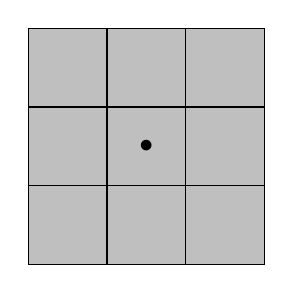
\begin{tikzpicture}
\draw [fill=lightgray] (0,0) rectangle  (3,3);
\node at (1.5,1.5) {$\bullet$};
\foreach \x in {0,1,2,3} {
\draw (\x,0) -- (\x,3);
\draw (0,\x) -- (3,\x);}
\end{tikzpicture}}
\end{center}

and
	\[
		K = \max\left\{ k | (A \ominus kB \neq \emptyset) \right\}
	\]

$K$ is the last iterative step before $A$ is eroded to an empty step. \\

Reconstruction can be achieved by
	\[
		A = \bigcup_{k=0}^{K}\left( S_k(A) \oplus kB \right)
	\]
\textbf{Problems:}
\begin{itemize}
	\item The resulting skeleton is not connected
	\item The skeleton is a bit thicker than it needs to be.
\end{itemize}
\end{multicols}

\subsubsection{Pruning\buchSeite{664}}
Pruning is a procedure that can remove parasitic components of a length below some threshold.\\
\begin{enumerate}
\item Find endpoints with a hit or miss transform with the following structuring elements. Remove the endpoints.
\begin{figure}[h!]
\centering
\begin{subfigure}[b]{0.45\textwidth}
\centering
\adjustbox{scale=0.5}{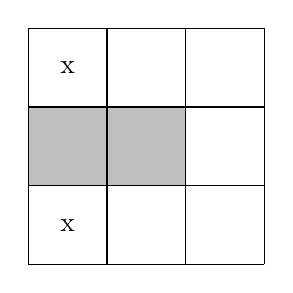
\begin{tikzpicture}
%\draw [fill=lightgray] (0,0) rectangle  (3,1);
\draw [fill=lightgray] (0,1) rectangle  (2,2);
\node at (0.5,0.5) {x};
\node at (0.5,2.5) {x};
\foreach \x in {0,1,2,3} {
\draw (\x,0) -- (\x,3);
\draw (0,\x) -- (3,\x);}
\end{tikzpicture}}
\caption{$B^1, B^2, B^3, B^4$ (rotated $90^\circ$)}
\end{subfigure}
\begin{subfigure}[b]{0.45\textwidth}
\centering
\adjustbox{scale=0.5}{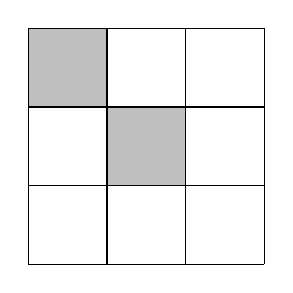
\begin{tikzpicture}
\draw [fill=lightgray] (0,3) rectangle  (1,2);
\draw [fill=lightgray] (1,1) rectangle  (2,2);
\foreach \x in {0,1,2,3} {
\draw (\x,0) -- (\x,3);
\draw (0,\x) -- (3,\x);}
\end{tikzpicture}}
\caption{$B^5, B^6, B^7, B^8$ (rotated $90^\circ$)}
\end{subfigure}
\caption{Pruning structuring elements}
\end{figure}
\item Repeat this. If you want to remove all spurs of length 3 or less, repeat for 3 times
\item Find the endpoints using the same structuring elements
\item Dilate the endpoints with a 3x3 structuring element and make a logical and with the original set
\end{enumerate}

\subsubsection{Morphological Reconstruction\buchSeite{667}}
\paragraph{Geodesic dilation and erosion\buchSeite{667}}
This is a transformation which uses two images and a structuring element
\begin{itemize}
\item F is the marker image
\item G is the mask image
\item Both are binary and F is a subset of G
\end{itemize}
Note that morphological reconstruction will always converge after a finite number of steps. \\

\textbf{Geodesic dilation}
\[
	D_G^{(1)}(F) = (F\oplus B)\cap G
\]
is the dilation of $F$ by $B$, where the result must stay inside $G$.
This can be repeated:
\begin{align*}
	D_G^{(0)}(F) = F \\
	D_G^{(1)}(F) = (F\oplus B)\cap G\\
	D_G^{(n)}(F) = D_G^{(1)}[D_G^{(n-1)}(F)]	&& \text{\tiny notice the recursive definition}
\end{align*}

\textbf{Geodesic erosion}
	\[
		E_G^{(0)}(F) = F
	\]
is the erosion of $F$ by $B$, where the result contains at least $G$.
\begin{align*}
	E_G^{(1)}(F) &= (F\ominus B)\cup G \\
	E_G^{(n)}(F) &= E_G^{(1)}[E_G^{(n-1)}(F)]
\end{align*}

\paragraph{Morphological reconstruction by dilation and by erosion\buchSeite{668}}
This is geodesic dilation/erosion until nothing changes.
\begin{align*}
    \text{Reconstruction by dilation:} \quad R_G^D(F)=D_G^{(k)} \quad \text{with} \quad D_G^{(k)}(F)=D_G^{(k+1)}(F)\\
    \text{Reconstruction by erosion:} \quad R_G^E(F)=E_G^{(k)} \quad \text{with} \quad E_G^{(k)}(F)=E_G^{(k+1)}(F)
\end{align*}

\paragraph{Sample applications\buchSeite{669}}
\textbf{Opening and closing by reconstruction}\\
Opening by reconstruction removes all small object, all others stay unchanged.
Closing by reconstruction closes gaps, the rest is unchanged. This is in contrast to morphological opening and closing, where the erosion removes the small objects and the dilation "sort of" reconstructs the other objects.\\
\begin{align*}
O_R^{(n)}(F)=R_F^D[(F\ominus nB)]\\
C_R^{(n)}(F)=R_F^E[(F\oplus nB)]
\end{align*}

\textbf{Filling holes in a binary image I}\\
Without needing a seed!\\
\[
	H = [R_F^D(F)]^C  \qquad  \text{with} \qquad \text{F}(x,y)=\begin{cases} 1-I(x,y) & \text{if (x,y) is on the border of I}\\
                                                             0 & \text{otherwise} \end{cases}
\]
\begin{figure}[h!]
\centering
\begin{subfigure}[b]{0.13\textwidth}
\centering
\adjustbox{scale=0.4}{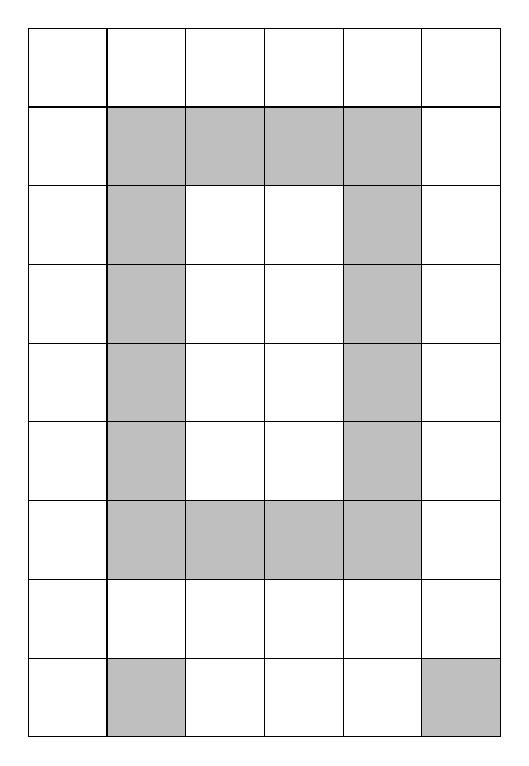
\begin{tikzpicture}
\draw [fill=lightgray] (1,2) rectangle  (2,8);
\draw [fill=lightgray] (2,2) rectangle  (4,3);
\draw [fill=lightgray] (5,8) rectangle  (4,2);
\draw [fill=lightgray] (4,7) rectangle  (2,8);
\draw [fill=lightgray] (5,0) rectangle  (6,1);
\draw [fill=lightgray] (1,0) rectangle  (2,1);

\foreach \x in {0,...,6} {
\draw (\x,0) -- (\x,9);}
\foreach \x in {0,...,9} {
\draw (0,\x) -- (6,\x);}
\end{tikzpicture}}
\caption{$I$}
\end{subfigure}
\begin{subfigure}[b]{0.13\textwidth}
\centering
\adjustbox{scale=0.4}{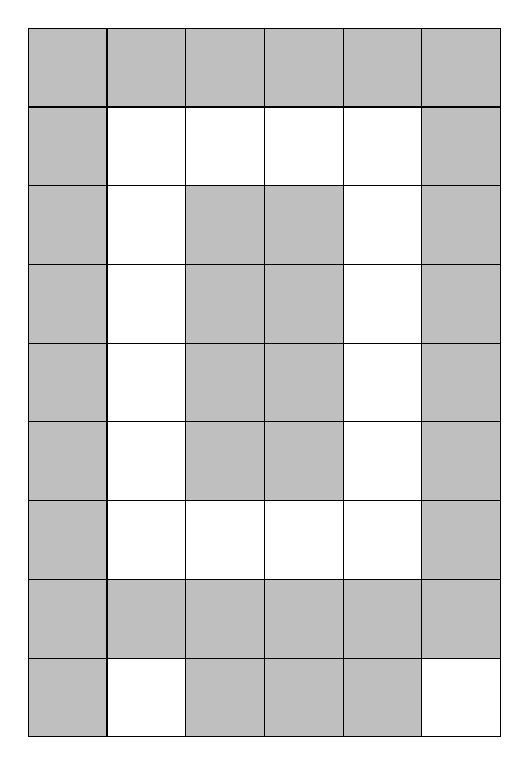
\begin{tikzpicture}
\draw [fill=lightgray] (0,0) rectangle (6,9);
\draw [fill=white] (1,2) rectangle  (2,8);
\draw [fill=white] (2,2) rectangle  (4,3);
\draw [fill=white] (5,8) rectangle  (4,2);
\draw [fill=white] (4,7) rectangle  (2,8);
\draw [fill=white] (5,0) rectangle  (6,1);
\draw [fill=white] (1,0) rectangle  (2,1);

\foreach \x in {0,...,6} {
\draw (\x,0) -- (\x,9);}
\foreach \x in {0,...,9} {
\draw (0,\x) -- (6,\x);}
\end{tikzpicture}}
\caption{$I^c$}
\end{subfigure}
\begin{subfigure}[b]{0.13\textwidth}
\centering
\adjustbox{scale=0.4}{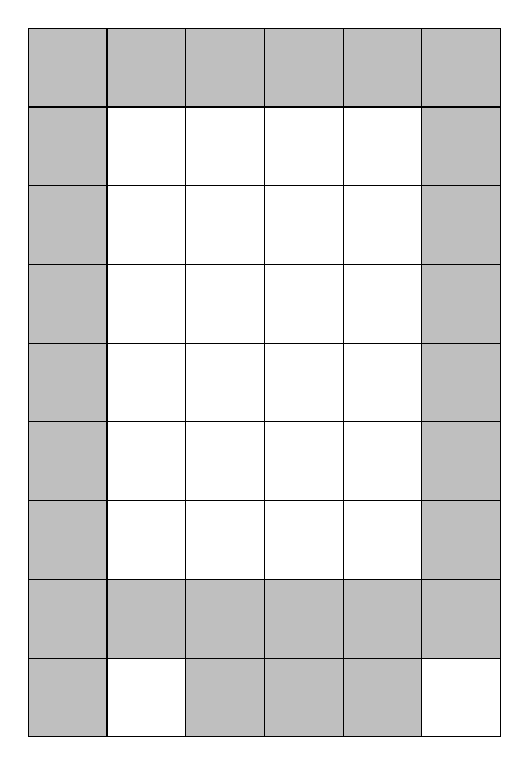
\begin{tikzpicture}
\draw [fill=lightgray] (0,0) rectangle (6,9);
\draw [fill=white] (1,2) rectangle  (5,8);
\draw [fill=white] (5,0) rectangle  (6,1);
\draw [fill=white] (1,0) rectangle  (2,1);

\foreach \x in {0,...,6} {
\draw (\x,0) -- (\x,9);}
\foreach \x in {0,...,9} {
\draw (0,\x) -- (6,\x);}
\end{tikzpicture}}
\caption{$F$}
\end{subfigure}
\begin{subfigure}[b]{0.13\textwidth}
\centering
\adjustbox{scale=0.4}{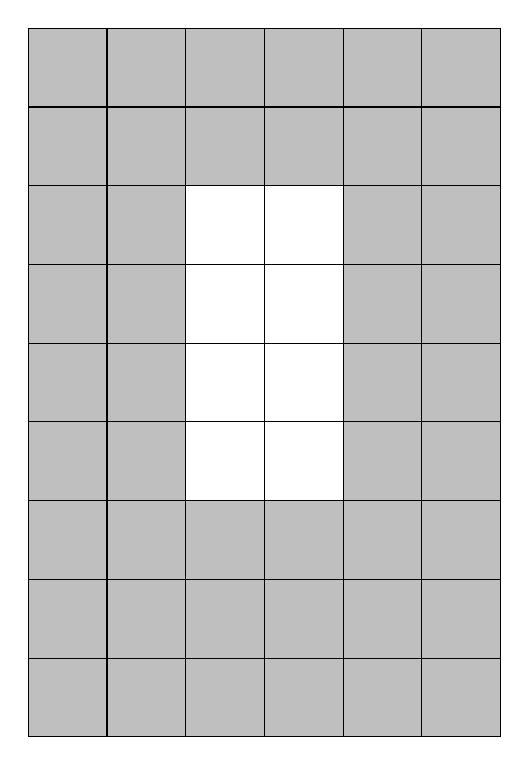
\begin{tikzpicture}
\draw [fill=lightgray] (0,0) rectangle (6,9);
\draw [fill=white] (2,3) rectangle  (4,7);

\foreach \x in {0,...,6} {
\draw (\x,0) -- (\x,9);}
\foreach \x in {0,...,9} {
\draw (0,\x) -- (6,\x);}
\end{tikzpicture}}
\caption{$C \oplus B$}
\end{subfigure}
\begin{subfigure}[b]{0.13\textwidth}
\centering
\adjustbox{scale=0.4}{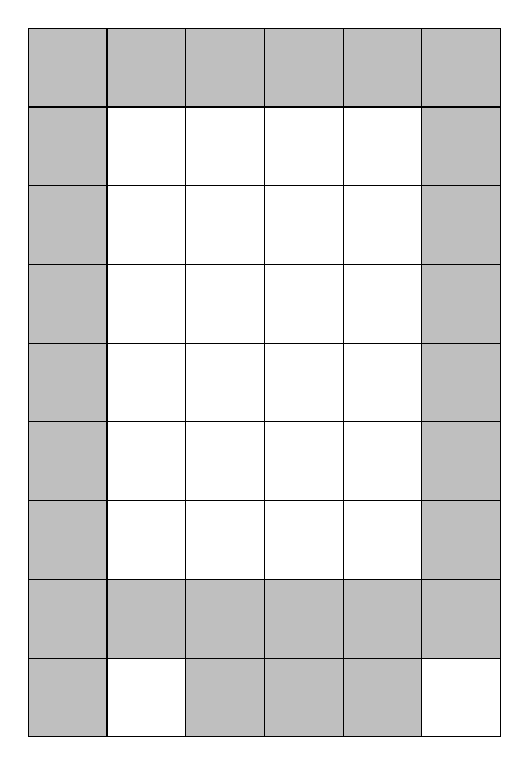
\begin{tikzpicture}
\draw [fill=lightgray] (0,0) rectangle (6,9);
\draw [fill=white] (1,2) rectangle  (5,8);
\draw [fill=white] (5,0) rectangle  (6,1);
\draw [fill=white] (1,0) rectangle  (2,1);

\foreach \x in {0,...,6} {
\draw (\x,0) -- (\x,9);}
\foreach \x in {0,...,9} {
\draw (0,\x) -- (6,\x);}
\end{tikzpicture}}
\caption{$C \oplus B \bigcap I^c$}
\end{subfigure}
\begin{subfigure}[b]{0.13\textwidth}
\centering
\adjustbox{scale=0.4}{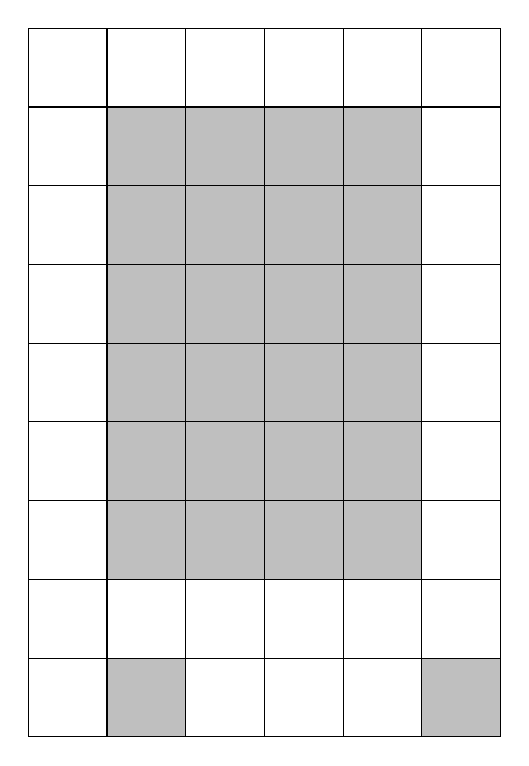
\begin{tikzpicture}
\draw [fill=lightgray] (1,2) rectangle  (5,8);
\draw [fill=lightgray] (5,0) rectangle  (6,1);
\draw [fill=lightgray] (1,0) rectangle  (2,1);

\foreach \x in {0,...,6} {
\draw (\x,0) -- (\x,9);}
\foreach \x in {0,...,9} {
\draw (0,\x) -- (6,\x);}
\end{tikzpicture}}
\caption{$H$}
\end{subfigure}
\begin{subfigure}[b]{0.13\textwidth}
\centering
\adjustbox{scale=0.4}{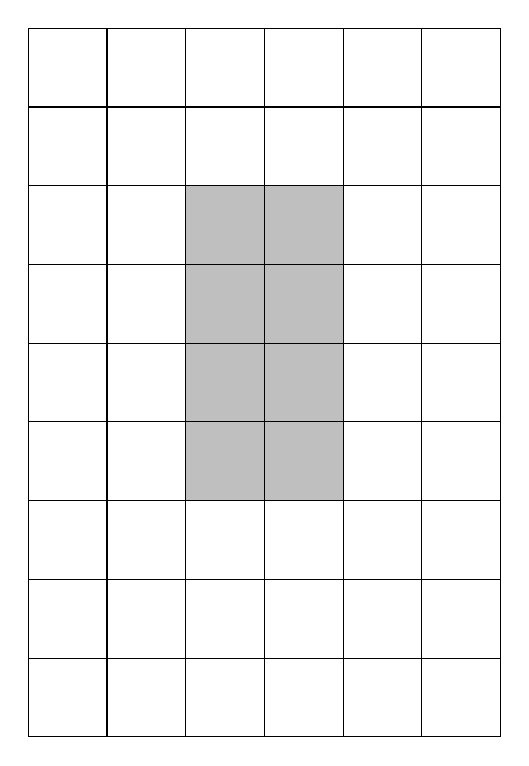
\begin{tikzpicture}
\draw [fill=lightgray] (2,3) rectangle  (4,7);

\foreach \x in {0,...,6} {
\draw (\x,0) -- (\x,9);}
\foreach \x in {0,...,9} {
\draw (0,\x) -- (6,\x);}
\end{tikzpicture}}
\caption{$H \bigcap I^c$}
\end{subfigure}
\caption{Hole Filling on a simple image}
\end{figure}

\textbf{Border clearing}\\
Remove object that touch the border.
\[
X = I-R_I^D(F)  \qquad  \text{with} \qquad \text{F}(x,y)=\begin{cases} I(x,y) & \text{if (x,y) is on the border of I}\\
0 & \text{otherwise} \end{cases}
\]

\subsection{Grayscale morphology\buchSeite{674}}
The fundamental operations dilation, erosion, opening and closing can be extended to gray scale. Hence the more advanced operations which are based on the above operations can be extended too. The structuring elements are also gray-scale. In practice, flat structuring elements are preferred.

\begin{figure}[h!]
\centering
\begin{subfigure}[b]{0.45\textwidth}
\centering
\adjustbox{scale=0.5}{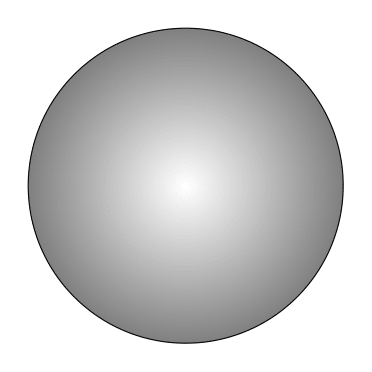
\includegraphics[width=5cm]{tikz/morphological/nonflatSE.png}}
\caption{Nonflat SE}
\end{subfigure}
\begin{subfigure}[b]{0.45\textwidth}
\centering
\adjustbox{scale=0.5}{\begin{tikzpicture}
\draw (0,0) circle (2);\end{tikzpicture}}
\caption{Flat SE}
\end{subfigure}\\
\begin{subfigure}[b]{0.45\textwidth}
\centering
\adjustbox{scale=0.5}{\begin{tikzpicture}
\draw (0,0) -- (0,2);
\draw (4,2) arc (0:180:2) ;
\draw (4,2) -- (4,0);
\end{tikzpicture}}
\caption{Intensity profile}
\end{subfigure}
\begin{subfigure}[b]{0.45\textwidth}
\centering
\adjustbox{scale=0.5}{\begin{tikzpicture}
\draw (0,0) -- (0,4) -- (4,4) -- (4,0);\end{tikzpicture}}
\caption{Intensity profile}
\end{subfigure}\\
\caption{Nonflat and flat structuring elements and corresponding horizontal intensity profiles through their center}
\end{figure}

\subsubsection{Erosion and Dilation\buchSeite{674}}
Erosion
\begin{align*}
	[f\ominus b](x,y)	&= \min_{(s,t)\in b} \{f(x+s,y+t)\}				& \text{Flat SE} \\
	[f\ominus b_N](x,y)	&= \min_{(s,t)\in b_n} \{f(x+s,y+t) -b_N(s,t)\}	& \text{Non-Flat SE}
\end{align*}

Dilation
\begin{align*}
	[f\oplus b](x,y)	&= \max_{(s,t)\in b} \{f(x-s,y-t)\}				& \text{Flat SE} \\
	[f\oplus b_N](x,y)	&= \max_{(s,t)\in b_N} \{f(x-s,y-t) +b_N(s,t)\}	& \text{Non-Flat SE}
\end{align*}

\subsubsection{Opening and Closing\buchSeite{680}}
Opening and closing are defined exactly the same as in the binary case:
\begin{align*}
	f \circ b = (f \ominus b) \oplus b &&
	f  \bullet b = (f \oplus b) \ominus b
\end{align*}

\subsubsection{Some Basic Gray-Scale Morphological Algorithms\buchSeite{682}}
\paragraph{Morphological smoothing\buchSeite{682}}
Opening suppresses bright details and closing suppresses dark details. They can be used in combination for image smoothing and/or noise suppression.
\paragraph{Morphological gradient\buchSeite{682}}
This operation results in an image where the edges are enhanced, not unlike a classical magnitude gradient image.
\[
	g=(f\oplus b)-(f\ominus b)
\]
\paragraph{Top-hat transformation\buchSeite{683}}
\[
	T_{hat}(f) = f -(f \circ b)
\]
The resulting image contains mostly bright details that are smaller than the structuring element.
\paragraph{Bottom-hat transformation\buchSeite{683}}
\[
	B_{hat}(f) = (f \bullet b)-f
\]
The resulting image contains mostly dark details, that are smaller than the structuring element.
\paragraph{Granulometry\buchSeite{685}}
The goal of granulometry is to find the particle size distribution in an image. Opening with a structuring element similar in shape as the particles but the size scaled from small to large. The biggest effect in the resulting opened image is, when the size of the structuring element changes from just too small to just too large. This effect can be measured by summing up the entire opened image, the surface area. Jumps in the change of surface area show the dominant particle sizes.
\paragraph{Textural segmentation\buchSeite{687}}
Figure 9.43\\
The goal of textural segmentation is, to segment the image into two textural regions. The basic idea is to remove the small circles with a structuring element larger than the small circle but smaller than the large circle. With a following opening fills the white patches between the large elements.
\subsubsection{Grayscale morphological reconstruction\buchSeite{688}}
Follows the definition for binary images.\\

\begin{multicols}{2}
\textbf{Geodesic dilation}
\begin{align*}
	D_g^{(1)}(f) = (f\oplus b)\wedge g\\
	D_g^{(n)}(f) = D_g^{(1)}[D_g^{n-1}(f)] g
\end{align*}
$\wedge$ denotes the point-wise minimum operator. \\

\textbf{Opening by reconstruction}
	\[
		O_R^{(n)} (f) = R_f^D \left[ (f \ominus nb) \right]
	\]

\textbf{Geodesic erosion}
\begin{align*}
	E_g^{(1)}(f) = (f\ominus b)\vee g\\
	E_g^{(n)}(f) = E_g^{(1)}[E_g^{(n-1)}(f)]
\end{align*}
$\vee$ denotes the point-wise maximum operator. \\

\textbf{Closing by reconstruction}
	\[
		C_R^{(n)} (f) = R_f^E \left[ (f \oplus nb) \right]
	\]
\end{multicols}
